%%%%%%%%%%%%%%%%%%%%%%%%%%%%%%%%%%%%%%%%%
% Thin Sectioned Essay
% LaTeX Template
% Version 1.0 (3/8/11)
%
% This template has been downloaded from:
% http://www.LaTeXTemplates.com
%
% Original Author:
% Nicolas Diaz (nsdiaz@uc.cl) with extensive modifications by:
% Vel (vel@latextemplates.com)
%
% License:
% CC BY-NC-SA 3.0 (http://creativecommons.org/licenses/by-nc-sa/3.0/)
%
%%%%%%%%%%%%%%%%%%%%%%%%%%%%%%%%%%%%%%%%%

%----------------------------------------------------------------------------------------
%	PACKAGES AND OTHER DOCUMENT CONFIGURATIONS
%----------------------------------------------------------------------------------------

\documentclass[a4paper, 11pt]{article} % Font size (can be 10pt, 11pt or 12pt) and paper size (remove a4paper for US letter paper)
\usepackage{hyperref}

\usepackage[protrusion=true,expansion=true]{microtype} % Better typography
\usepackage{graphicx} % Required for including pictures
\usepackage{wrapfig} % Allows in-line images
\usepackage{tablefootnote} % to display footnotes in tables
\usepackage{threeparttable}
\usepackage[toc,page]{appendix}
\usepackage{multirow}
\usepackage{color}

\usepackage{mathpazo} % Use the Palatino font
\usepackage[T1]{fontenc} % Required for accented characters
\linespread{1.05} % Change line spacing here, Palatino benefits from a slight increase by default

\newcommand{\hls}{HLS\,J0918+5142}
\makeatletter
%\renewcommand\@biblabel[1]{\textbf{#1.}} % Change the square brackets for each bibliography item from '[1]' to '1.'
\renewcommand{\@listI}{\itemsep=0pt} % Reduce the space between items in the itemize and enumerate environments and the bibliography

\renewcommand{\maketitle}{ % Customize the title - do not edit title and author name here, see the TITLE block below
\begin{flushleft} % Right align
{\LARGE\@title} % Increase the font size of the title

\vspace{50pt} % Some vertical space between the title and author name

{\large\@author} % Author name
\\\@date % Date

\vspace{40pt} % Some vertical space between the author block and abstract
\end{flushleft}
}

%
% PAGE STYLE
%
\setlength{\textwidth}{16cm}
\setlength{\textheight}{23cm}
\oddsidemargin +0.5cm
\evensidemargin +0.5cm
\topmargin 0.1cm

%----------------------------------------------------------------------------------------
%	TITLE
%----------------------------------------------------------------------------------------

\title{\textbf{NIKA2 research note}\\   
\textsc{NIKA2 Commissioning results v1.0}} % Subtitle


\author{NIKA2 team % Author
\\{\textit{NIKA2 collaboration}}} % Institution

\date{\today} % Date



%----------------------------------------------------------------------------------------

\begin{document}

\maketitle % Print the title section
%
%
%
\tableofcontents

%----------------------------------------------------------------------------------------
%	SENSITIVITIES
%----------------------------------------------------------------------------------------
\section{Sensitivities}
\label{se:nefd}
%%
%%
%%      SECTION: SENSITIVITY
%%

\begin{figure}
\begin{center}
%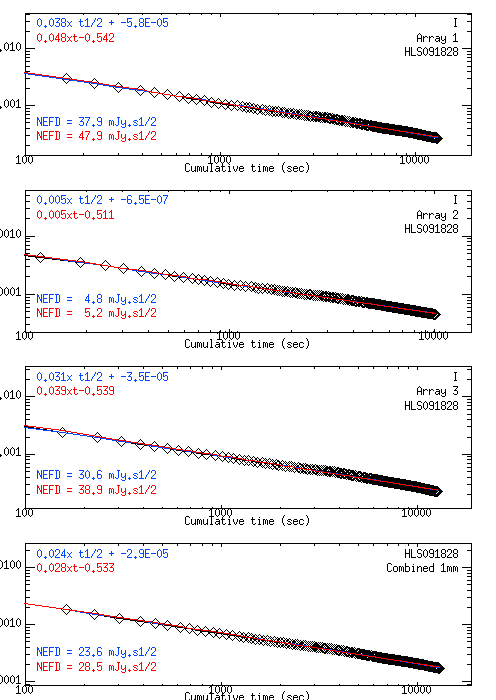
\includegraphics[clip, angle=0, scale =
%  0.5]{Figures/NEFD_HLS091828_20170226s415_FXDC0C1_GaussPhot.png}
\includegraphics[clip, angle=0, scale = 0.5]{Figures/nefd_mpfit_HLS091828.eps}
\caption{Kids Xcalib with fixed fwhm 12.5 and 18.5, \hls.}
\label{fig:nefd_vs_t}
\end{center}
\end{figure}

{\bf The specs/goals ``NEFD on X \% of pixels'' should be understood as : we have
XX\% valid pixels, and with these pixels, we have an NEFD of YY. We should not
discard some fraction of our pixels and estimate an NEFD on this subset.}\\

\hls is moderately faint source, expected to be below 100~mJy at 1mm and
XX~mJy at 2mm {\bf check values in NIKA1 paper + use SED for predictions in
  NIKA2's bands}. This source was chosen for its flux and its availability during
Run9 for long integration. It has been observed for XX hours in total over three
nights.


\subsection{Observations}

As part of the NIKA2 Science Verification that took place in February 2017, we
observed an area of 185~arcmin$^2$, centered on \hls, (a lensed dusty galaxy at
z=5.24 \cite{combes2012}) during about 9~hours. The scans were 8x5~arcmin$^2$,
alternatively oriented in (ra,dec), (dec,ra), (az,el), (el,az). This leads to
the coverage presented on Fig.~\ref{fig:hls_cov} and effective integration times
on \hls\ of $\sim 2.4$\,hours at 2\,mm and $\sim 1.7$\,hours at 1.2\,mm (the
difference comes from the different density of detectors across the field of
view for the two bands). This allowed us to reach $1\sigma$ sensitivities of
about 0.3~mJy at 1.2\,mm and 0.1~mJy at 2\,mm on \hls. The integration time in a
map pixel $t_p$ of size $r\times r$~arcsec$^2$ is given by the number of hits in
this pixel $N_p$, divided by the sampling frequency $\nu$. This estimate is not
the time $t_{obs}$ that enters the definition of the NEFD and which is the time
spent by the matrix ``overall'' on the region where we give the
sensitivity. Indeed, we must account for the density of KIDs in the focal plane
compared to the map resolution : assume there are two KIDs per map pixel, then
$t_p = 2 t_{obs}$. A contrario, if the KIDs are sparsely distributed accross the
focal plane, some map pixels are empty while they are physically covered by the
FOV. Let's call $g$ the spacing between KIDs in arcsec in the FOV, we thus have:

\begin{eqnarray}
t_{obs} &=& \frac{t_p}{N_{kids\,per\,pix}} \nonumber\\
&=& \frac{t_p}{N_{kids}/N_{pix}} \nonumber\\
&=& \frac{t_p\pi R_{FOV}^2/r^2}{\pi R_{FOV}^2/g^2} \nonumber\\
&=&t_p g^2r^2
\end{eqnarray}

\begin{figure}[htbp]
\begin{center}
\includegraphics[clip, angle=0, scale = 0.30]{Figures/hls_sensit_1mm.eps}
\includegraphics[clip, angle=0, scale = 0.30]{Figures/hls_sensit_2mm.eps}
\caption{Sensitivity per beam in mJy at 1 and 2mm}
\label{fig:hls_cov}
\end{center}
\end{figure}


\subsection{Data processing}

The data were decorrelated using the {\tt common-monde-one-block} method
(cf.~\ref{se:cm1blck}), masking a disk of 60~arcsec radius centered \hls.  The
scans have been combined with standard inverse noise weighting. The noise in
each map pixel is derived from the rms of the background corrected by the square
root of the number of observations per pixel (N1). If the noise was perfectly
gaussian, the distribution of the map signal over this noise estimate (far from
the source) would be a normalized gaussian. In practice, this leads to gaussians
that 1.6 and 1.5 larger. We therefore increase our noise estimate (N1) by these
factors to derive our final estimates. Should the extra sources that pop up in
the field contribute to this estimate, they would only make our estimate more
conservative.

\subsection{NEFD Methods 1 and 2: deep integration}

These data can be used to derive the NEFD in several ways. One is to fit the
evolution of the uncertainty on the flux of the source $\sigma_\phi$ with the
integration time. Another one is to produce jackknife maps with the data and to
measure the uncertainty on the flux in the end, while estimating the time of
integration. Results are summarized in
Tab.~\ref{tab:nefd}. Fig.~\ref{fig:nefd_vs_t} shows the decrease of the
uncertainty on the measured flux at the center of the map as a function of
time. We either fit a power law or fix the power law to -0.5 and fit only the
amplitude. Uncertainties on these values have been estimated via a bootstrap
method: we randomize the scans and derive the standard deviation of the average
of $n$ scans for any $n$ between 1 and the total number of scans. This gives us
an estimate of the uncertainty on $\sigma_\phi$ for a time of integration
corresponding to $n$ scans. Strictly speaking, all the scans do not have the
exact same duration, but the difference is negligible here.

\begin{table}
\begin{tabular}{|l|l|l|l|l|}
\hline
Array & Free power law & Fixed power law $t^{-0.5}$ & Jackknife & Instrument \\
\hline
A1       & $47.9$ mJy.s$^{-0.54}$ & $37.9$ mJy.s$^{1/2}$ & 35.6 mJy.s$^{1/2}$ & $33.3$ (5) mJy.s$^{1/2}$\\
A2       & $5.2$  mJy.s$^{-0.51}$ & $4.8$  mJy.s$^{1/2}$ & 5.7  mJy.s$^{1/2}$ & $5.8$  (5) mJy.s$^{1/2}$\\
A3       & $38.9$ mJy.s$^{-0.54}$ & $30.6$ mJy.s$^{1/2}$ & 30.4 mJy.s$^{1/2}$ & $28.4$ (4) mJy.s$^{1/2}$\\
A1 \& A3 & $28.5$ mJy.s$^{-0.53}$ & $23.6$ mJy.s$^{1/2}$ & 22.4 mJy.s$^{1/2}$ & $21.1$ (3) mJy.s$^{1/2}$\\
\hline
\end{tabular}
\label{tab:nefd}
\caption{Noise integration with observation time and associated derivations of
  the NEFD. These values do not account for the extra {\color{red} \bf XXXX \%}
  uncertainty on absolute calibration.}
\end{table}
%       33.325263       5.2024647
%       28.397230       4.5723151
%       21.143376       4.1538804
%       5.7628233       3.3094792


\begin{figure}
\begin{center}
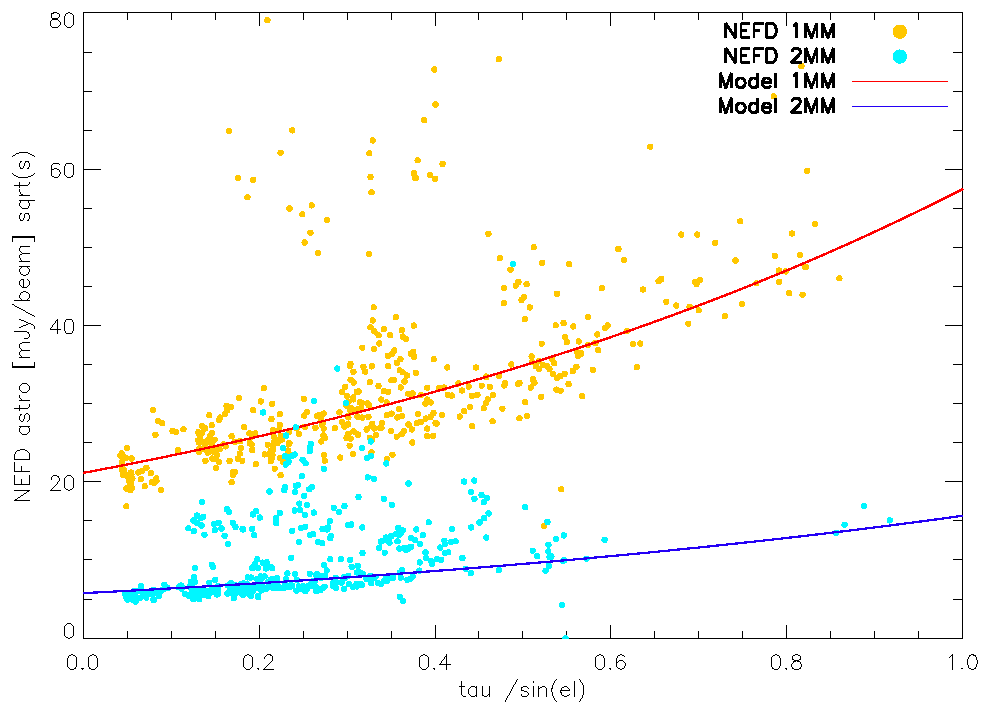
\includegraphics[clip, angle=0, scale =0.8]{Figures/NEFDIndScans/nefd_tau_run22.pdf}
\caption{Astronomer NEFD as a function of atmospheric background for the 1 (orange dots) and 2 (cyan dots) mm channels. We also show the expected NEFD evolution with atmospheric background (red and blue curves)}
\label{fig:nefdvsbackground}
\end{center}
\end{figure}

\subsection{NEFD Method 3: scan NEFD vs opacity and air mass}
\begin{figure}
\begin{center}
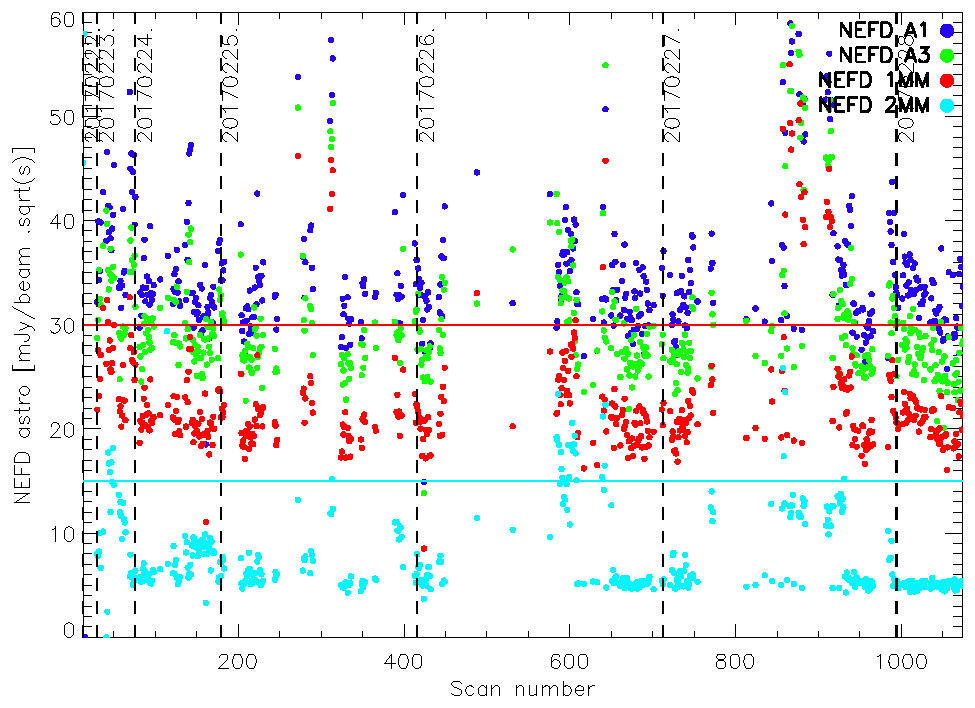
\includegraphics[clip, angle=0, scale =0.8]{Figures/NEFDIndScans/nefd_evol_run22.pdf}
\caption{Evolution of the measured instrument NEFD across scans for N2R9.}
\label{fig:nefdvsscans}
\end{center}
\end{figure}

\begin{figure}
\begin{center}
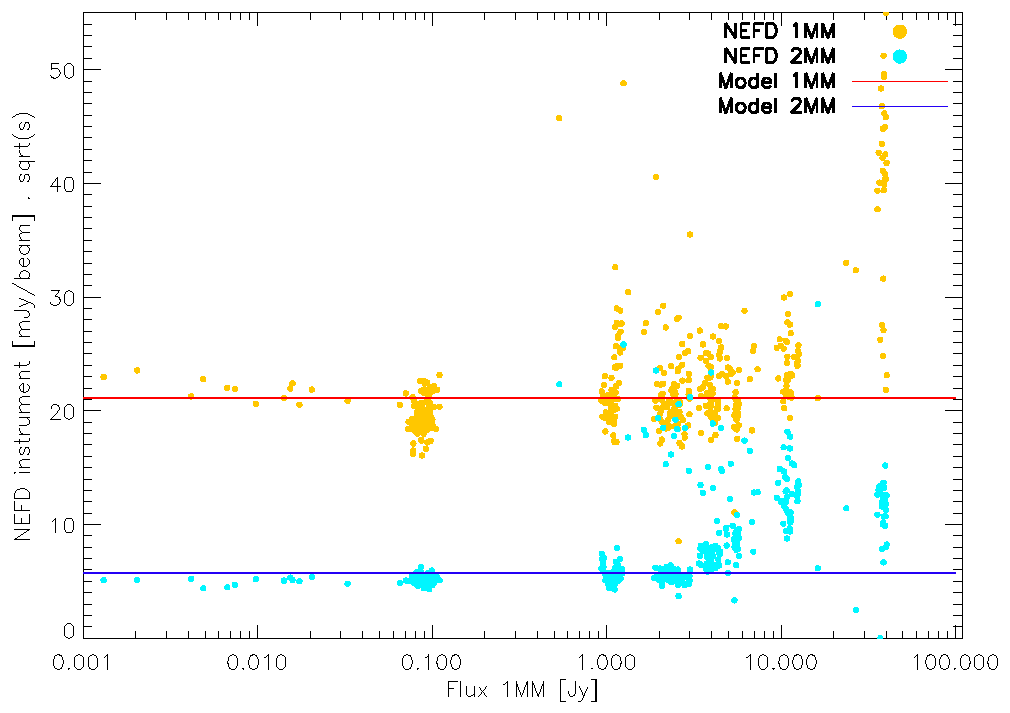
\includegraphics[clip, angle=0, scale =0.8]{Figures/NEFDIndScans/nefd_flux1mm_run22.pdf}
\caption{Measured instrument NEFD as a function of the flux of the source.}
\label{fig:nefdvsflux}
\end{center}
\end{figure}
\begin{figure}
\begin{center}
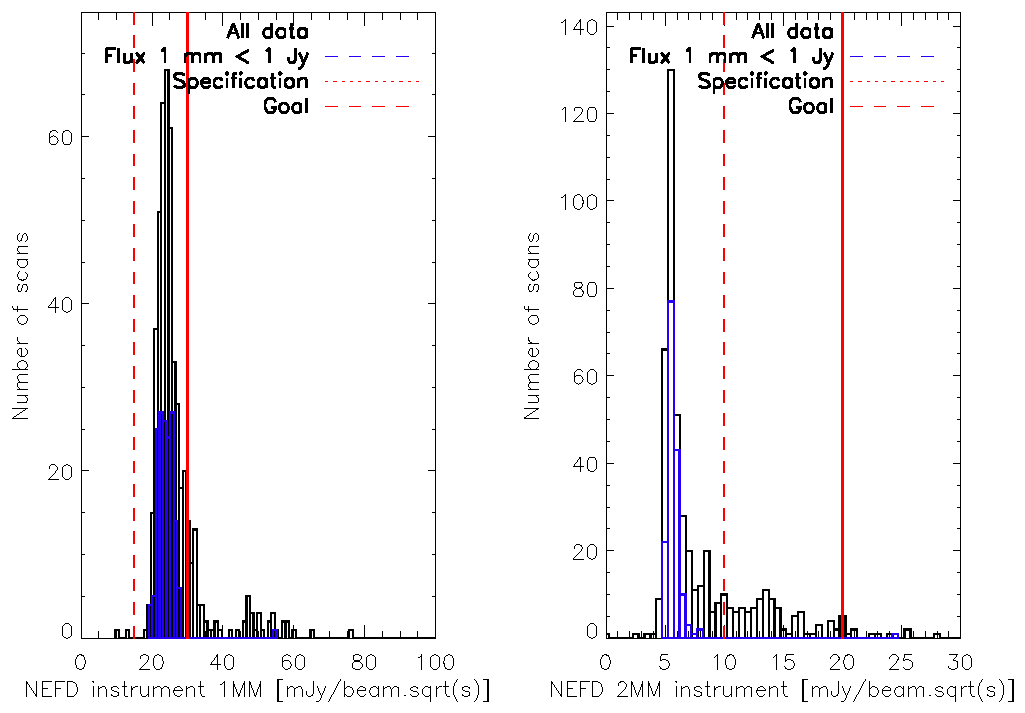
\includegraphics[clip, angle=0, scale =0.8]{Figures/NEFDIndScans/hist_nefd_ref_run22.pdf}
\caption{Histogram of the measured reference NEFD across the N2R9 for the 1 (right) and 2 (left) mm channels.}
\label{fig:nefdhist}
\end{center}
\end{figure}
 

In this section we investigate the astronomer NEFD as a function of the atmospheric opacity and air mass. Figure~\ref{fig:nefdvsbackground} shows the measured NEFD, which we refer to as astronomer NEFD, for the 1 and 2 mm as a function of the measured atmospheric background in terms of $\tau/sin(El)$. The atmospheric opacity was computed as discussed in Section~\ref{se:opacities}. We observe that the increase of the astronomer NEFD is in agreement with what we would expect for background dominated sensitivity. We observe however some significant deviations from the curve. To investigate this issue we also show in Figure~\ref{fig:nefdvsscans} the evolution of the background corrected NEFD, hereafter instrument NEFD, across the N2R9 campaign for arrays A1 (blue), A3 (green) and A2 (cyan), and for the combination of A1 and A3 (red). We globally obseve stable NEFD across the run, with A1 sensitivity being worse than for A3. We also show the measured instrument NEFD as a function of the flux of the source in the 1 mm channel in Figure~\ref{fig:nefdvsflux}. We observe that the observed deviations in the instrument NEFD correspond mainly to the large flux source scans. This is more obvious in Figure~\ref{fig:nefdhist} where we present the histogram of the measured NEFD for 2 mm of pwv and at a elevation of 60 degrees, hereafter, reference NEFD, for the 1 and 2 mm channels.





%
\begin{thebibliography}{99}
  
\bibitem[{Pardo {et~al.} 2002}]{Pardo2002}
Pardo, J.~R., Cernicharo, J. \& Serabyn, E., 2002, 
IEEE Transactions on Antennas and Propagation 49, 1683

\bibitem{Dempsey}(Dempsey et al 2013)
\bibitem{Knapp} (Knapp et al 1994)
\bibitem{Tafoya}(Tafoya et al 2004)

\bibitem{beloche}
\url{http://www.lesia.obspm.fr/perso/emmanuel-lellouch/mars/index.php}

\bibitem{gith-Haussel-Note}
\url{https://github.com/haussel/photometry/blob/master/notebooks/planet_fluxes.ipynb}

\bibitem{PLCK-LII}(Planck intermediate results LII, Planck
Collaboration in press)

\bibitem{gith-Haussel}
\url{https://github.com/haussel/photometry}.

\bibitem{NASAHorizon}
\url{https://ssd.jpl.nasa.gov/horizons.cgi}

\bibitem{ESAmodel}
\url{https://www.cosmos.esa.int/web/herschel/calibrator-models}

\bibitem{krips}M. Krips, talk at the 8th 
IRAM Millimeter Interferometry School, Grenoble (France),  October 2012, and
privae communication.\\
\url{http://www.iram.fr/IRAMFR/IS/IS2012/presentations/krips-fluxcalibration.pdf}
\bibitem{durand}Durand's PhD Thesis at
Universit\'e Grenoble Alpes, 2008

\bibitem{Calvo16}
M. Calvo {\it et al.},  
Journal of Low Temperature Physics 184 (2016) 816-823 
%arXiv:1601.02774 

\bibitem{NIKA2-Tech}
 R.~Adam {\it et al.}, arXiv:1707.00908  
 
%NIKA
\bibitem{Monfardini11}    A. Monfardini {\it et al.}, The Astrophysical Journal Supplement 194 (2011)  24 
\bibitem{Bourrion12}    O. Bourrion {\it et al.}, JINST 11 (2016) P11001 
\bibitem{Calvo13}    M. Calvo {\it et al.}, Astron.\ Astrophys.\  {\bf 551} (2013) L12
\bibitem{Monfardini13} A. Monfardini {\it et al.}, JLTP 176 (2014) 787
    
 
\bibitem{Catalano:2014nml}
  A.~Catalano {\it et al.},
  %``Performance and calibration of the NIKA camera at the IRAM 30 m telescope,''
  Astron.\ Astrophys.\  {\bf 569} (2014) A9.
%  doi:10.1051/0004-6361/201423557
  %%CITATION = doi:10.1051/0004-6361/201423557;%%
  %5 citations counted in INSPIRE as of 16 Feb 2016
  

  
 
%\cite{Ritacco:2016due}
\bibitem{Ritacco:2016due}
  A.~Ritacco {\it et al.},
  %``Polarimetry at millimeter wavelengths with the NIKA camera: calibration and performance,''
  Astron.\ Astrophys.\  {\bf 599} (2017) A34
%  doi:10.1051/0004-6361/201629666
%  [arXiv:1609.02042 [astro-ph.IM]].
  %%CITATION = doi:10.1051/0004-6361/201629666;%%
  %2 citations counted in INSPIRE as of 21 Jul 2017
  
\bibitem{Bracco}
  A.~Bracco {\it et al.},
  %``Probing changes of dust properties along a chain of solar-type prestellar and protostellar cores in Taurus with NIKA,''
  Astron.\ Astrophys.\  {\bf 604} (2017) A52
  %%CITATION = doi:10.1051/0004-6361/201731117;%%


\bibitem{Adam:2013ufa}
  R.~Adam {\it et al.},
  %``First observation of the thermal Sunyaev-Zel\u2019dovich effect with kinetic inductance detectors,''
  Astron.\ Astrophys.\  {\bf 569} (2014) A66
%  doi:10.1051/0004-6361/201322902
%  [arXiv:1310.6237 [astro-ph.CO]].
  %%CITATION = doi:10.1051/0004-6361/201322902;%%
  %8 citations counted in INSPIRE as of 16 Feb 2016
  

\bibitem{Adam:2014wxa}
  R.~Adam {\it et al.},
  %``Pressure distribution of the high-redshift cluster of galaxies CL J1226.9+3332 with NIKA,''
  Astron.\ Astrophys.\  {\bf 576} (2015) A12
%  doi:10.1051/0004-6361/201425140
%  [arXiv:1410.2808 [astro-ph.CO]].
  %%CITATION = doi:10.1051/0004-6361/201425140;%%
  %5 citations counted in INSPIRE as of 16 f�vr. 2016
  


%\cite{Adam:2015bba}
\bibitem{Adam:2015bba}
  R.~Adam {\it et al.},
  %``High angular resolution Sunyaev-Zel\u2019dovich observations of MACS J1423.8+2404 with NIKA: Multiwavelength analysis,''
  Astron.\ Astrophys.\  {\bf 586} (2016) A122
%  doi:10.1051/0004-6361/201527616
%  [arXiv:1510.06674 [astro-ph.CO]].
  %%CITATION = doi:10.1051/0004-6361/201527616;%%
  %12 citations counted in INSPIRE as of 21 Jul 2017
  
  
\bibitem{Adam:2016abn}
  R.~Adam {\it et al.},
  %``Mapping the kinetic Sunyaev-Zel\u2019dovich effect toward MACS J0717.5+3745 with NIKA,''
  Astron.\ Astrophys.\  {\bf 598} (2017) A115
%  doi:10.1051/0004-6361/201629182
%  [arXiv:1606.07721 [astro-ph.CO]].
  %%CITATION = doi:10.1051/0004-6361/201629182;%%
  %6 citations counted in INSPIRE as of 21 Jul 2017  



%\cite{Ruppin:2016rnt}
\bibitem{Ruppin:2016rnt}
  F.~Ruppin {\it et al.},
  %``Non-parametric deprojection of NIKA SZ observations: Pressure distribution in the Planck-discovered cluster PSZ1\u2009G045.85+57.71,''
  Astron.\ Astrophys.\  {\bf 597} (2017) A110
%  doi:10.1051/0004-6361/201629405
%  [arXiv:1607.07679 [astro-ph.CO]].
  %%CITATION = doi:10.1051/0004-6361/201629405;%%
  %3 citations counted in INSPIRE as of 21 Jul 2017
  
%\cite{Adam:2017mlj}
\bibitem{Adam:2017mlj}
  R.~Adam {\it et al.},
  %``Mapping the hot gas temperature in galaxy clusters using X-ray and Sunyaev-Zel'dovich imaging,''
  arXiv:1706.10230 [astro-ph.CO].
  %%CITATION = ARXIV:1706.10230;%%
%\cite{Adam:2016abn}



  

%\cite{Romero:2017xri}
\bibitem{Romero:2017xri}
  C.~Romero {\it et al.},
  %``A multi-instrument non-parametric reconstruction of the electron pressure profile in the galaxy cluster CLJ1226.9+3332,''
  arXiv:1707.06113 [astro-ph.CO].
  %%CITATION = ARXIV:1707.06113;%%
  
  
%\cite{Comis:2016bpf}
\bibitem{Comis:2016bpf}
  B.~Comis {\it et al.},
  %``High angular resolution SZ observations with NIKA and NIKA2,''
  arXiv:1605.09549 [astro-ph.CO].
  %%CITATION = ARXIV:1605.09549;%%
  %3 citations counted in INSPIRE as of 26 Jul 2017
  
  
 








\end{thebibliography}


%----------------------------------------------------------------------------------------

\end{document}
